\chapter{进入保护模式} \label{CHpm}

前面我们看到,通过一些很简单的代码,我们做到了启动一个微型系统,加载文件系统中的文件进入内存并运行的功能。应该注意的是,在前面的代码中我们使用的内存空间都很小。我们看一下~boot.bin~和~LOADER.BIN~的大小就能感觉出来(当然,可执行文件小未必使用内存空间小,但是这两个文件也太小了~\smiley)。

\begin{Command}
$ ls -l boot.bin LOADER.BIN 
-rwxr-xr-x 1 solrex solrex 512 2008-04-26 16:34 boot.bin
-rwxr-xr-x 1 solrex solrex  15 2008-04-26 16:34 LOADER.BIN
\end{Command}

boot.bin~是~512~个字节(其中还有我们填充的内容,实际指令只有~480~个字节),而~LOADER.BIN~更过分,只有~15~个字节大小。可想而知这两个文件在内存中能使用多大的空间吧。如果读者有些汇编语言经验的话,就会发现我们在前面的程序中使用的存储器寻址都是在实模式下进行的,即:由段寄存器(cs,~ds:~16-bit)配合段内偏移地址(16-bit)来定位一个实际的~20-bit~物理地址,所以我们前面的程序最多支持~$2^{20} = 2^{10}*2^{10} = 1024*1024$ bytes = 1MB~的寻址空间。

哇,~1MB~不小了,我们的操作系统加一起连~1KB~都用不到,~1MB~寻址空间足够了。但是需要考虑到的一点是,就拿我们现在用的~1.44MB的(已经被淘汰的)软盘标准来说,如果软盘上某个文件超过~1MB~,我们的操作系统就没办法处理了。那么如果以后把操作系统安装到硬盘上之后呢?我们就没办法处理稍微大一点的文件了。

所以我们要从最原始的~Intel 8086/8088 CPU~的实模式中跳出来,进入~Intel 80286~之后系列~CPU~给我们提供的保护模式。这还将为我们带来其它更多的好处,具体内容请继续往下读。

\section{实模式和保护模式}

\BOXED{0.9\textwidth}{
\danger\\ 如果您需要更详细的知识,也许您更愿意去读 Intel 的手册,本节内容主要集中在:\href{http://download.intel.com/design/processor/manuals/253668.pdf}{Intel\textregistered~64 and IA-32 Architectures Software Developer's Manual, Volume 3A: System Programming Guide}, 第~2~章和第~3~章.\enddanger
}

\subsection{一段历史}

Intel~公司在~1978~年发布了一款~16~位字长~CPU: 8086~,最高主频~5 MHz $\sim$ 10 MHz~,集成了~29,000~个晶体管,这款在今天感觉像玩具一样的~CPU~却是奠定今天~Intel PC~芯片市场地位的最重要的产品之一。虽然它的后继者~8088~,加强版的~8086~(增加了一个~8~比特的外部总线)才是事实上的~IBM~兼容机(PC,个人电脑)雏形的核心,但人们仍然习惯于用~8086~作为厂商标志代表~Intel~。

因为受到字长(16~位)的限制,如果仅仅使用单个寄存器寻址,~8086~仅仅能访问~64KB($2^{16}$)~的地址空间,这显然不能满足一般要求,而当时~1MB($2^{20}$)~对于一般的应用就比较足够了,所以~8086~使用了~20~位的地址线。

在~8086~刚发布的时候,没有“实模式”这个说法,因为当时的~Intel CPU~只有一种模式。在~Intel~以后的发布中,~80286~引入了“保护模式”寻址方式,将~CPU~的寻址范围扩大到~16($2^{24}$) MB~,但是~80286~仍然是一款~16~位~CPU~,这就限制了它的广泛应用。但是“实模式”这个说法,就从~80286~开始了。

接下来的发展就更快了,1985~年发布的~i386~首先让~PC CPU~进入了~32~位时代,由此而带来的好处显而易见,寻址能力大大增强,但是多任务处理和虚拟存储器的需求仍然推动着~i386~向更完善的保护模式发展。下面我们来了解一下“实模式”和“保护模式”的具体涵义。

\subsection{实模式}

实模式(real mode),有时候也被成为实地址模式(real address mode)或者兼容模式(compatibility mode)是~Intel 8086 CPU~以及以其为基础发展起来的~x86~兼容~CPU~采用的一种操作模式。其主要的特点有:20~比特的分段访问的内存地址空间(即~1~MB~的寻址能力);程序可直接访问~BIOS~中断和外设;硬件层不支持任何内存保护或者多任务处理。~80286~之后所有~x86 CPU~在加电自举时都是首先进入实模式;~80186~以及之前的~CPU~只有一种操作模式,相当于实模式。

\subsection{保护模式}

保护模式(protected mode),有时候也被成为保护的虚拟地址模式(protected virtual address mode),也是一种~x86~兼容~CPU~的工作模式。保护模式为系统软件实现虚拟内存、分页机制、安全的多任务处理的功能支持,还有其它为操作系统提供的对应用程序的控制功能支持,比如:特权级、实模式应用程序兼容、虚拟~8086~模式。

\subsection{实模式和保护模式的寻址模式}

前面提到过,实模式下的地址线是~20~位的,所以实模式下的寻址模式使用分段方式来解决~16~位字长机器提供~20~位地址空间的问题。这个分段方法需要程序员在编制程序的过程中将存储器划分成段,每个段内的地址空间是线性增长的,最大可达~64K($2^16$),这样段內地址就可以使用~16~位表示。段基址(~20-bit~)的最低~4~位必须是~0~,这样段基址就可以使用~16~位段地址来表示,需要时将段地址左移~4~位就得到段起始地址。除了便于寻址之外,分段还有一个好处,就是将程序的代码段、数据段和堆栈段等隔离开,避免相互之间产生干扰。

当计算某个单元的物理地址时,比如汇编语言中的一个~Label~,就通过段地址(~16-bit~)左移~4~位得到段基址(~20-bit~),再加上该单元~(Label)~的段內偏移量(~16-bit~)来得到其物理地址(~20-bit~),如图~\ref{rm_addr}~所示。

\begin{figure*}[!t]
\centerline{\subfloat[实模式寻址模型]{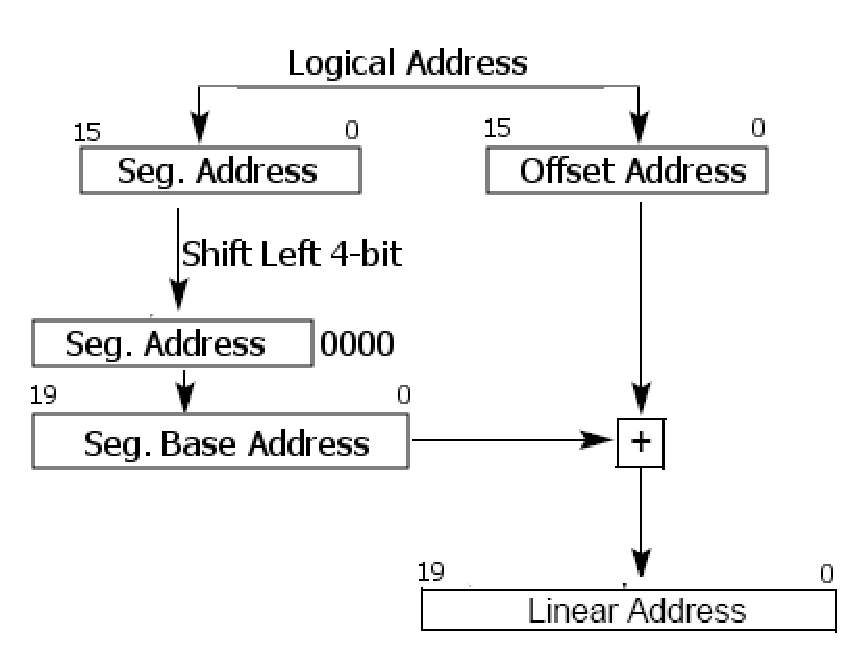
\includegraphics[width=.48\textwidth,keepaspectratio]{rm_addr}%
\label{rm_addr}}
\hfil
\subfloat[保护模式寻址模型]{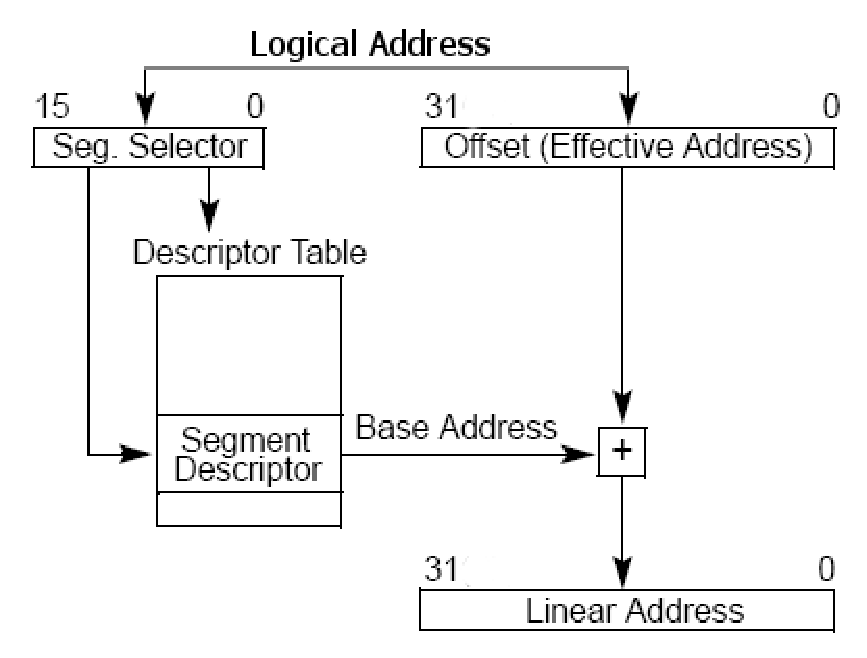
\includegraphics[width=.48\textwidth,keepaspectratio]{protected_seg}%
\label{protected_seg}}}
\caption{实模式与保护模式寻址模型比较}
\label{real_vs_pro}
\end{figure*}

一般情况下,段地址会被放在四个段寄存器中,即:代码段~CS,数据段~DS,堆栈段~SS~和附加段~ES~寄存器。这样在加载数据或者控制程序运行的时候,只需要一个偏移量参数,CPU~会自动用对应段的起始地址加上偏移量参数来得到需要的地址。(后继~CPU~又加上了两个段寄存器~FS~和~GS~,不过使用方式是基本一样的。)

由此可见,实模式的寻址模式是很简单的,就是用两个~16~位逻辑地址(段地址:偏移地址)组合成一个~20~位物理地址,而保护模式的寻址方式就要稍微复杂一点了。

\BOXED{0.9\textwidth}{
Intel~的~CPU~在保护模式下是可以选择打开分页机制的,但为了简单起见,我们先不开启分页机制,所以下面的讲解针对只有分段机制的保护模式展开。
}

在保护模式下,每个单元的物理地址仍然是由逻辑地址表示,但是这个逻辑地址不再由(段地址:偏移地址)组成了,而是由(段选择子:偏移地址)表示。这里的偏移地址也变成了~32~位的,所以段空间也比实模式下大得多。偏移地址的意思和实模式下并没有本质不同,但段地址的计算就要复杂一些了,如图~\ref{protected_seg}~所示。段基址(Segment Base Address)被存放在段描述符(Segment Descriptor)中,GDT(Global Descriptor Table,全局段选择子表)是保存着所有段选择子的信息,段选择子(Segment Selector)是一个指向某个段选择子的索引。

如图~\ref{protected_seg}~所示,当我们计算某个单元的物理地址时,只需要给出(段选择子:偏移地址),CPU~会从~GDT~中按照段选择子找到对应的段描述符,从段描述符中找出段基址,将段基址加上偏移量,就得到了该单元的物理地址。

\section{与保护模式初次会面}

介绍完了保护模式和实模式的不同,下面我们就尝试一下进入保护模式吧。在上一章我们已经实现了用启动扇区加载引导文件,所以这里我们就不用再去管启动扇区的事情了,下面的修改均在~loader.S~中进行。上一章的~loader.S~仅仅实现在屏幕的上方中间打印了一个~\code{L}~,下面我们的~loader.S~要进入保护模式来打印一些新东西。

首先,我们来理清一下应该如何进入保护模式:

\begin{enumerate}
  \item 我们需要一个~GDT。由于保护模式的寻址方式是基于~GDT~的,我们得自己写一个~GDT~数据结构并将其载入到系统中。
  \item 我们需要为进入保护模式作准备。由于保护模式和实模式运行方式不同,在进入保护模式之前,我们需要一些准备工作。
  \item 我们需要一段能在保护模式下运行的代码 demo,以提示我们成功进入了保护模式。
\end{enumerate}

下面我们就来一步步完成我们的第一个保护模式~loader~。

\subsection{GDT~数据结构}

要写~GDT,首先得了解~GDT~的数据结构。GDT~实际上只是一个存储段描述符的线性表(可以理解成一个段描述符数组),对它的要求是其第一个段描述符置为空,因为处理机不会去处理第一个段描述符,所以理解~GDT~的数据结构难点主要在于理解段描述符的数据结构。

段描述符主要用来为处理机提供段位址,段访问控制和状态信息。图~\ref{seg_desc}~显示了一个基本的段描述符结构:

\FIG{段描述符}{seg_desc}{.9\textwidth}

看到上面那么多内容,是不是感觉有点儿恐怖啊!其实简单的来看,我们现在最关注的是段基址,就是图~\ref{seg_desc}~中标记为~Base~的部分。可以看到,段基址在段描述符中被分割为三段存储,分别是:Base 31:24, Base 23:16, Base Address 15:0,把这三段拼起来,我们就得到了一个~32~位的段基址。

有了段基址,就需要有一个界限来避免程序跑丢发生段错误,这个界限就是图~\ref{seg_desc}~中标记为~Limit~的部分,将~Seg. Limit 19:16~和~Segment Limit 15:0~拼起来我们就得到了一个~20~位的段界限,这个界限就是应该是段需要的长度了。

下面还要说的就是那个~D/B Flag~,D/B~代表~Default Operation Size~,0~代表~16~位的段,1~代表~32~位的段。为了充分利用~CPU~,我们当然要设置为~32~位模式了。剩下那些乱七八糟的~Flag~呢,无非就是提供段的属性(代码段还是数据段?只读还是读写?),我们将在第~\ref{CHpm_desattr}~节为大家详细介绍。

这些东西那么乱,难道要每次一点儿一点儿地计算吗?放心,程序员自有办法,请看下面的程序:

\VerbatimInput[fontfamily=tt,fontsize=\footnotesize,frame=lines, framerule=0.4mm, numbers=left, numbersep=3pt, tabsize=2, firstline=56, lastline=70]{../src/chapter3/1/pm.h}
\codecaption{自动生成段描述符的宏定义(节自 chapter3/1/pm.h)}\label{CHpm_descm}

图~\ref{CHpm_descm}~中所示,就是自动生成段描述符的汇编宏定义。我们只需要给宏~Descriptor~三个参数:Base(段基址), Limit(段界限[段长度]), Attr(段属性),Descriptor~就会自动将三者展开放到段描述符中对应的位置。看看我们在程序中怎么使用这个宏:

\VerbatimInput[fontfamily=tt,fontsize=\footnotesize,frame=lines, framerule=0.4mm, numbers=left, numbersep=3pt, tabsize=2, firstline=21, lastline=26]{../src/chapter3/1/loader.S}
\codecaption{自动生成段描述符的宏使用示例(节自 chapter3/1/loader.S)}\label{CHpm_descmu}

图~\ref{CHpm_descmu}~中,就利用~Descriptor~宏生成了三个段描述符,形成了一个~GDT。注意到没有,第一个段描述符是空的(参数全为~0)。这里~LABEL\_DESC\_CODE32~的段基址为~0~是因为我们无法确定它的准确位置,它将在运行期被填入。

有人可能会产生疑问,段基址和段界限什么意思我们都知道了,那段属性怎么回事呢?~DA\_C, DA\_32, DA\_DRW~都是什么东西啊?是这样的,为了避免手动一个一个置段描述符中的~Flag~,我们预先定义了一些常用属性,用的时候只需要将这些属性加起来作为宏~Descriptor~的参数,就能将段描述符中的所有~flag~置上(记得~C~语言中~fopen~的参数吗?)。这些属性的定义如下(没必要细看,用的时候再找即可):

\VerbatimInput[fontfamily=tt,fontsize=\footnotesize,frame=lines, framerule=0.4mm, numbers=left, numbersep=3pt, tabsize=2, firstline=11, lastline=55]{../src/chapter3/1/pm.h}
\codecaption{预先设置的段属性(节自 chapter3/1/pm.h)}\label{CHpm_segattr}

\subsection{保护模式下的~demo}

为什么把这节提前到第~\ref{CHpm_secloadgdt}~节前讲呢?因为要写入~GDT~正确的段描述符,首先要知道段的信息,我们就得先准备好这个段:

\VerbatimInput[fontfamily=tt,fontsize=\footnotesize,frame=lines, framerule=0.4mm, numbers=left, numbersep=3pt, tabsize=2, firstline=83, lastline=99]{../src/chapter3/1/loader.S}
\codecaption{第一个在保护模式下运行的 demo(节自 chapter3/1/loader.S)}\label{CHpm_demo1}

其实这个段的作用很简单,通过操纵视频段数据,在屏幕中间打印一个红色的"P"(和我们前面使用~BIOS~中断来打印字符的方式有所不同)。

\subsection{加载~GDT} \label{CHpm_secloadgdt}

GDT~所需要的信息我们都知道了,GDT~表也通过图~\ref{CHpm_descmu}~中的代码实现了。那么,我们应该向~GDT~中填入缺少的信息,然后载入~GDT~了。将~GDT~载入处理机是用~\code{lgdt}~汇编指令实现的,但是~\code{lgdt}~指令需要存放~GDT~的基址和界限的指针作参数,所以我们还需要知道~GDT~的位置和~GDT~的界限:

\VerbatimInput[fontfamily=tt,fontsize=\footnotesize,frame=lines, framerule=0.4mm, numbers=left, numbersep=3pt, tabsize=2, firstline=22, lastline=63]{../src/chapter3/1/loader.S}
\codecaption{加载~GDT(节自 chapter3/1/loader.S)}\label{CHpm_loadgdt}

图~\ref{CHpm_loadgdt}~中~\code{GdtPtr}~所指,即为~GDT~的界限和基址所存放位置。某段描述符对应的~GDT~选择子,就是其段描述符相对于~GDT~基址的索引(在我们例子里~GDT~基址为~\code{LABEL\_GDT}~指向的位置)。这里需要注意的是,虽然我们在代码中写:

\begin{Command}
.set SelectorCode32, (LABEL_DESC_CODE32 - LABEL_GDT)
\end{Command}
但实际上段选择子在使用时需要右移~3~个位作为索引去寻找其对应的段描述符,段选择子的右侧~3~个位是为了标识~TI~和~RPL~的,如图~\ref{descriptor}~所示,这点我们将在第~\ref{CHpm_ldt}~节和第~\ref{CHpm_desattr}~节中详细介绍。但是这里为什么能直接用地址相减得到段选择子呢?因为段选择子的大小是~8 bit~,用地址相减的话,最右侧三个位就默认置~0~了。

在图~\ref{CHpm_loadgdt}~中所示的代码,主要干了两件事:第一,将图~\ref{CHpm_demo1}~所示~demo~的段基址放入~GDT~中对应的段描述符中;第二,将~GDT~的基址放到~\code{GdtPtr}~所指的数据结构中,并加载~\code{GdtPtr}~所指的数据结构到~GDTR~寄存器中(使用~\code{lgdt}~指令)。

\subsection{进入保护模式}

进入保护模式前,我们需要将中断关掉,因为保护模式下中断处理的机制和实模式是不一样的,不关掉中断可能带来麻烦。使用~\code{cli}~汇编指令可以清除所有中断~flag。

由于实模式下仅有~20~条地址线:A0, A1, \ldots, A19,所以当我们要进入保护模式时,需要打开~A20~地址线。打开~A20~地址线有至少三种方法,我们这里采用~IBM~使用的方法,通常被称为:“Fast A20 Gate”,即修改系统控制端口~92h~,因为其端口的第~1~位控制着~A20~地址线,所以我们只需要将~0b00000010~赋给端口~92h~即可。

当前面两项工作完成后,我们就可以进入保护模式了。方法很简单,将~cr0~寄存器的第~0~位~PE~位置为~1~即可使~CPU~切换到保护模式下运行。

\VerbatimInput[fontfamily=tt,fontsize=\footnotesize,frame=lines, framerule=0.4mm, numbers=left, numbersep=3pt, tabsize=2, firstline=64, lastline=77]{../src/chapter3/1/loader.S}
\codecaption{进入保护模式(节自 chapter3/1/loader.S)}\label{CHpm_enablepm}

\subsection{特别的混合跳转指令}

虽然已经进入了保护模式,但由于我们的~CS~寄存器存放的仍然是实模式下~16~位的段信息,要跳转到我们的~demo~程序并不是那么简单的事情。因为~demo~程序是~32~位的指令,而我们现在仍然运行的是~16~位的指令。从~16~位的代码段中跳转到~32~位的代码段,不是一般的~near~或~far~跳转指令能解决得了的,所以这里我们需要一个特别的跳转指令。在这条指令运行之前,所有的指令都是~16~位的,在它运行之后,就变成~32~位指令的世界。

在~Intel~的手册中,把这条混合跳转指令称为~far jump(ptr16:32)~,在~NASM~手册中,将这条指令称为~Mixed-Size Jump~,我们就沿用~NASM~的说法,将这条指令称为混合字长跳转指令。NASM~提供了这条指令的汇编语言实现:
\begin{Command}
jmp dword 0x1234:0x56789ABC
\end{Command}
但是很遗憾的是,GAS~没有提供这条指令的实现,所以我们必须用~.byte~伪代码直接写二进制指令(如图~\ref{CHpm_mixedjmp}),比较庆幸的是,我们也只需要用到它一次。

\VerbatimInput[fontfamily=tt,fontsize=\footnotesize,frame=lines, framerule=0.4mm, numbers=left, numbersep=3pt, tabsize=2, firstline=77, lastline=82]{../src/chapter3/1/loader.S}
\codecaption{混合字长跳转指令(节自 chapter3/1/loader.S)}\label{CHpm_mixedjmp}

执行这条混合字长的跳转指令时,CPU~就会用段选择子~\code{SelectorCode32}~去寻找~GDT~中对应的段,由于段偏移是~0~,所以~CPU~将跳转到图~\ref{CHpm_demo1}~中~demo~程序的开头。为了方便阅读,整个~loader.S~的代码附在图~\ref{CHpm_loader1}~中:

\VerbatimInput[fontfamily=tt,fontsize=\footnotesize,frame=lines, framerule=0.4mm, numbers=left, numbersep=3pt, tabsize=2, firstline=1, lastline=99]{../src/chapter3/1/loader.S}
\codecaption{chapter3/1/loader.S (节自 chapter3/1/loader.S)}\label{CHpm_loader1}

\subsection{生成镜像并测试}

使用与第~\ref{CHsmall_test}~节完全相同的方法,我们可以将代码编译并将~LOADER.BIN~拷贝到镜像文件中。利用最新的镜像文件启动~VirtualBox~我们得到图~\ref{vb_run_5}~。

可以看到,屏幕的左侧中央打出了一个红色的~P~,这就是我们那个在保护模式下运行的简单~demo~所做的事情,这说明我们的代码是正确的。从实模式迈入保护模式,这只是一小步,但对于我们的操作系统来说,这是一大步。从此我们不必再被限制到~20~位的地址空间中,有了更大的自由度。

\FIG{第一次进入保护模式}{vb_run_5}{0.75\textwidth}

\section{段式存储}

如果您仔细阅读了图~\ref{protected_seg}~,您就会发现图中并未提到~GDT~,而是使用的~Descriptor Table(DT)~。这是因为对于~x86~架构的~CPU~来说,~DT~总共有两个:我们上节介绍过的~GDT~和下面要介绍的~LDT~。这两个描述符表构成了~x86 CPU~段式存储的基础。顾名思义,~GDT~作为全局的描述符表,只能有一个,而~LDT~作为局部描述符表,就可以有很多个,这也是以后操作系统给每个任务分配自己的存储空间的基础。

\subsection{LDT~数据结构} \label{CHpm_ldt}

\FIG{段描述符数据结构}{descriptor}{0.6\textwidth}

事实上,~LDT~和~GDT~的差别非常小,~LDT~段描述符的数据结构和图~\ref{seg_desc}~所示是一样的。所不同的就是,~LDT~用指令~\code{lldt}~来加载,并且指向~LDT~描述符项的段选择子的~TI~位置必须标识为~1~,如图~\ref{descriptor}~所示。这样,操作系统才会从当前的~LDT~中去寻找对应的段描述符。

但这里值得注意的一点是:GDT~是由线性空间里的地址定义的,即~\code{lgdt}~指令的参数是一个线性空间的地址;而~LDT~是由~GDT~中的一个段描述符定义的,即~\code{lldt}~指令的参数是~GDT~中的一个段选择子。这是因为在加载~GDT~之前寻址模式是实模式的,而加载~GDT~后寻址模式变成保护模式寻址,将~LDT~作为~GDT~中的段使用,也方便操作系统在多个~LDT~之间切换。

\subsection{描述符属性} \label{CHpm_desattr}

我们在介绍图~\ref{seg_desc}~时,并没有完全介绍段描述符的各个~Flag~和可能的属性,这一小节就用来专门介绍段描述符的属性,按照图~\ref{seg_desc}~中的~Flag~从左向右的顺序:

\begin{itemize}
\item{\textbf{G}}: G(Granularity,粒度):如果~G flag~置为~0~,段的大小以字节为单位,段长度范围是~$1 byte\sim 1 MB$~;如果~G flag~置为~1~,段的大小以~4 KB~为单位,段长度范围是~$4 KB \sim 4 GB$~。
\item{\textbf{D/B}}:D/B(Default operation size/Default stack pionter size and/or upper Bound, 默认操作大小),其意思取决于段描述符是代码段、数据段或者堆栈段。该~flag~置为~0~代表代码段/数据段为~16~位的;置为~1~代表该段是~32~位的。
\item{\textbf{L}}:L(Long, 长),~L flag~是~IA-32e(Extended Memory 64 Technology)~模式下使用的标志。该~flag~置为~1~代表该段是正常的~64~位的代码段;置为~0~代表在兼容模式下运行的代码段。在~IA-32~架构下,该位是保留位,并且永远被置为~0~。
\item{\textbf{AVL}}:保留给操作系统软件使用的位。
\item{\textbf{P}}:P(segment-Present,段占用?) flag~用于标志段是否在内存中,主要供内存管理软件使用。如果~P flag~被置为~0~,说明该段目前不在内存中,该段指向的内存可以暂时被其它任务占用;如果~P flag~被置为~1~,说明该段在内存中。如果~P flag~为~0~的段被访问,处理机会产生一个~segment-not-present(\#NP)~异常。
\item{\textbf{DPL}}:DPL(Descriptor Privilege Level)域标志着段的优先级,取值范围是从~0$\sim$3(2-bit)~,0~代表着最高的优先级。关于优先级的作用,我们将在下节讨论。
\item{\textbf{S}}:S(descriptor type) flag~标志着该段是否系统段:置为~0~代表该段是系统段;置为~1~代表该段是代码段或者数据段。
\item{\textbf{Type}}:Type~域是段描述符里最复杂的一个域,而且它的意义对于代码/数据段描述符和系统段/门描述符是不同的,下面我们用两张图表来展示当~Type~置为不同值时的意义。

\begin{center}\begin{longtable}{c|c|c|c|c|c|l}
\caption[]{代码/数据段描述符的~Type~属性列表}\label{code_data_types}\\
\hline
\multicolumn{5}{c|}{\textbf{Type Field}} & \textbf{Descriptor Type} & \textbf{Description}\bigstrut\\
\cline{1-5}
\textbf{Decimal} & \textbf{11} & \textbf{10} & \textbf{9} & \textbf{8} & & \\
        &    &  \textbf{E} & \textbf{W} & \textbf{A} & & \\
\hline
0 & 0 & 0 & 0 & 0 & Data & Read-Only\\
1 & 0 & 0 & 0 & 1 & Data & Read-Only, Accessed\\
2 & 0 & 0 & 1 & 0 & Data & Read/Write\\
3 & 0 & 0 & 1 & 1 & Data & Read/Write, Accessed\\
4 & 0 & 1 & 0 & 0 & Data & Read-Only, Expand-down\\
5 & 0 & 1 & 0 & 1 & Data & Read-Only, Expand-down, Accessed\\
6 & 0 & 1 & 1 & 0 & Data & Read/Write, Expand-down\\
7 & 0 & 1 & 1 & 1 & Data & Read/Write, Expand-down, Accessed\\
\hline
        &    &  \textbf{C} & \textbf{R} & \textbf{A} & & \\
\hline
8 & 1 & 0 & 0 & 0 & Code & Execute-Only\\
9 & 1 & 0 & 0 & 1 & Code & Execute-Only, Accessed\\
10 & 1 & 0 & 1 & 0 & Code & Execute/Read\\
11 & 1 & 0 & 1 & 1 & Code & Execute/Read, Accessed\\
12 & 1 & 1 & 0 & 0 & Code & Execute-Only, Conforming\\
13 & 1 & 1 & 0 & 1 & Code & Execute-Only, Conforming, Accessed\\
14 & 1 & 1 & 1 & 0 & Code & Execute/Read-Only, Conforming\\
15 & 1 & 1 & 1 & 1 & Code & Execute/Read-Only, Conforming, Accessed\\
\hline
\end{longtable}\end{center}

\end{itemize}



